\subsubsection{Szczegóły modyfikacji algorytmu LAM}
Algorytm ten bez dodatkowego warunku na skojarzenie wierzchołków (linia $35$) zwykle tworzyłby grafy typu gwiazda, co oznacza,
że powstawałaby część wierzchołków o bardzo wysokim stopniu.
To powodowałoby, że zmniejszony graf nie przypominałby początkowego grafu.
Warunek ten został dodany przez autorów artykułu \cite{weighted_maching} i mówi, że
skojarzenie wierzchołka $a$ z wierzchołkiem $b$ może zaistnieć tylko wtedy, jeśli ich sumaryczna
waga nie przekracza dwukrotności najmniejszej wagi wierzchołka w grafie
zsumowanej z największą wagą wierzchołka w grafie.
\begin{equation}
w_{a} + w_{b} \leq w_{highest} + 2 \cdot w_{lowest}
\label{eq:condition1}
\end{equation}
Warunek \ref{eq:condition1} powoduje, że nawet jeśli rozpatrujemy skojarzenie wierzchołka o relatywnie wysokiej wadze, to ma on szansę
zostać skojarzony jedynie z wierzchołkiem o wadze niskiej, co prowadzi do równiejszych wag w grafie.
Przy dalszych etapach zmniejszania grafu trudniej spełnić
warunek na skojarzenie wierzchołków - pojawia się więcej różnorodności w kwestii wag wierzchołków grafu, spada
więc liczba udanych skojarzeń przypadających na wywołanie.
W momencie, kiedy zbyt mało par jest kojarzonych podczas pojedynczego wywołania, warunek ten jest osłabiany poprzez
zwiększenie dopuszczalnej sumarycznej wagi wierzchołka $a$ oraz $b$.

Warunek stworzony przez autorów artykułu \cite{weighted_maching} okazał się nie działać w kontekście obszarów
niepodzielnych.
W tym celu stworzony został nowy, zmodyfikowany warunek \ref{eq:condition3}, który jest warunkiem \ref{eq:condition1}
rozszerzonym o $discount$ (wzór \ref{eq:condition2}).
\begin{equation}
discount = \frac{t}{T \cdot \frac{w_{highest}}{w_{lowest} + 1} \cdot \log(number\_of\_partitions)}
\label{eq:condition2}
\end{equation}
Jeśli $discount > 1$ wtedy przypisywaną ma wartość 1.
$T$ to przewidywana liczba wywołań algorytmu LAM.
Obliczana jest jako liczba dzieleń liczby wierzchołków grafu przez liczbę dwa, potrzebna do uzyskania liczby wierzchołków mniejszej
lub równej docelowej liczby partycji.
$t$ to licznik wywołań algorytmu LAM (linia $2$).
Z użyciem $discountu$ powstał zmodyfikowany przeze mnie warunek na skojarzenie wierzchołków $a$ i $b$:
\begin{equation}
w_{a} + w_{b} \leq discount \cdot (w_{highest} + 2 \cdot w_{lowest})
\label{eq:condition3}
\end{equation}
Niedziałanie poprzedniego warunku, jest spowodowane faktem,
że w początkowej fazie algorytmu, tuż po zamianie wejściowej siatki na graf,
wszystkie obszary niepodzielne zamieniane są na pojedyncze wierzchołki.
Waga dla wierzchołków reprezentujących obszary niepodzielne jest równa sumie wag wierzchołków, które do nich należą.
Oryginalny algorytm LAM został zaprojektowany z założeniem o równomiernym budowaniu skojarzeń ze względu na wagi wierzchołków w grafie
od samego początku.
W warunku na skojarzenie wierzchołków bierze pod uwagę wierzchołek z aktualnie największą wagą
oraz aktualnie najmniejszą wagą w grafie.
Warunek ten funkcjonuje poprawnie, jeśli graf jest wedle niego zmniejszany równomiernie od samego początku, kiedy wagi wszystkich
wierzchołków w grafie mają taką samą wartość lub niemal taką samą wartość.
W momencie, w którym na samym początku pojawiają się wierzchołki o dużych wagach (z powodu zamiany wierzchołków
należących do obszarów niepodzielnych na pojedyncze wierzchołki o wyższych wagach) warunek \ref{eq:condition1} zaczyna
działać niepoprawnie.
W szczególnym przypadku, jeśli taki obszar zajmuje więcej niż połowę całej siatki
(rysunek \ref{im:discount}) niemal każde skojarzenie dwóch wierzchołków, z których żaden z nich nie jest wierzchołkiem
reprezentującym obszar niepodzielny, będzie dozwolone.
Każdy z takich wierzchołków ma bowiem wagę mniejszą niż suma podwojonej najmniejszej wagi wierzchołka w grafie oraz największej
wagi wierzchołka w grafie.
Warunek \ref{eq:condition1} jest więc niemal zawsze spełniony.
W tego typu przypadkach realny podział odbywa się tak naprawdę poza obszarem niepodzielnym, ponieważ wiemy, że obszar
niepodzielny będzie na końcu jedną partycją, a jako że jest największym wierzchołkiem w grafie - nie będzie mógł tworzyć
wielu skojarzeń.
Prowadzi to do tego, że obszary kojarzone są w sposób niezachowujący równomiernych pól jak na rysunku \ref{im:discount}(b).
W efekcie w skład wielu partycji wchodzi tylko jeden wierzchołek.

Zaproponowana przeze mnie modyfikacja (wzór \ref{eq:condition2}), polegająca na dodaniu $discountu$,
wzmacnia warunek
i powoduje bardziej równomierne (ze względu na wagi) łączenie się wierzchołków.
$discount$ zależny jest od liczby iteracji - osłabia się w czasie.
Im późniejsza iteracja tym bliższy jest wartości $1$,
a więc zmierza do oryginalnego warunku \ref{eq:condition1}.
Ważne jest jednak, że w kluczowych, początkowych wywołaniach algorytmu LAM pozwala na równomierne skojarzenia.
Efekt działania warunku widoczny jest na rysunku \ref{im:discount}.
\vspace{8mm}
\begin{figure}[h]
\centering
\begin{subfigure}{.5\textwidth}
    \centering
    \fbox{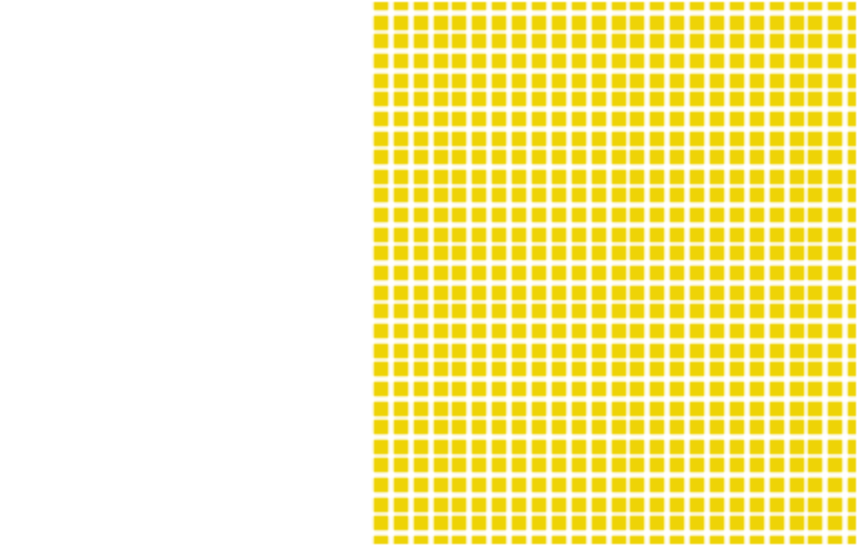
\includegraphics[width=0.7\textwidth]{images/discount1}}
    \caption[short]{siatka do partycjonowania}
\end{subfigure}%
\begin{subfigure}{.5\textwidth}
    \centering
    \fbox{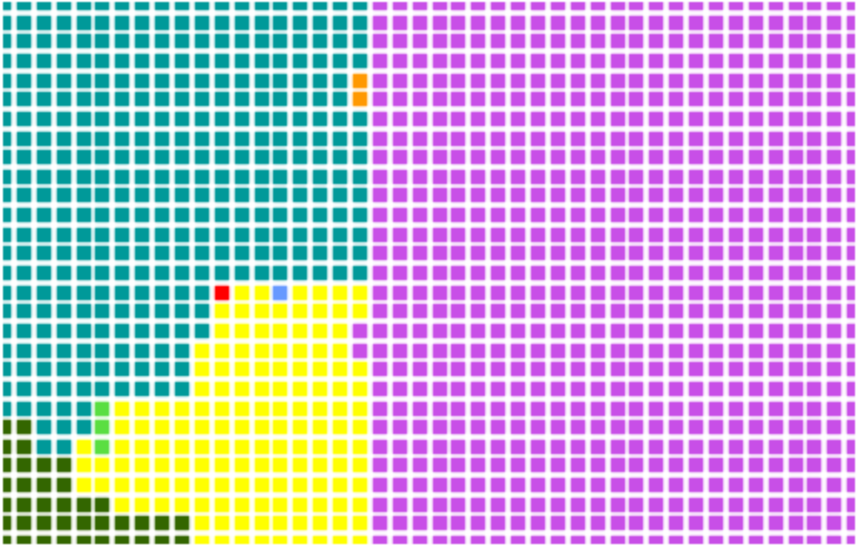
\includegraphics[width=0.7\textwidth]{images/discount2}}
    \caption[short]{partycjonowanie 1 bez użycia discountu}
\end{subfigure}
\begin{subfigure}{.5\textwidth}
    \centering
    \fbox{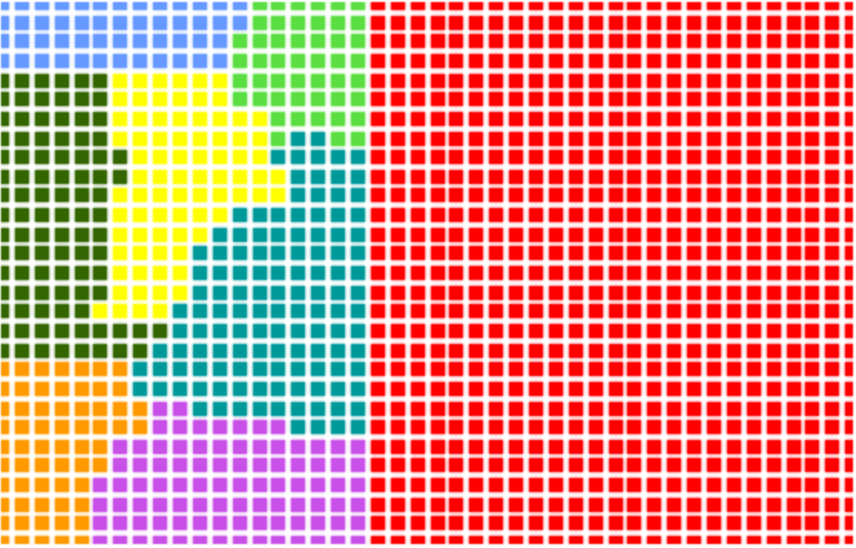
\includegraphics[width=0.7\textwidth]{images/discount3}}
    \caption[short]{partycjonowanie 2 z użyciem discountu}
\end{subfigure}%
\begin{subfigure}{.5\textwidth}
    \centering
    \fbox{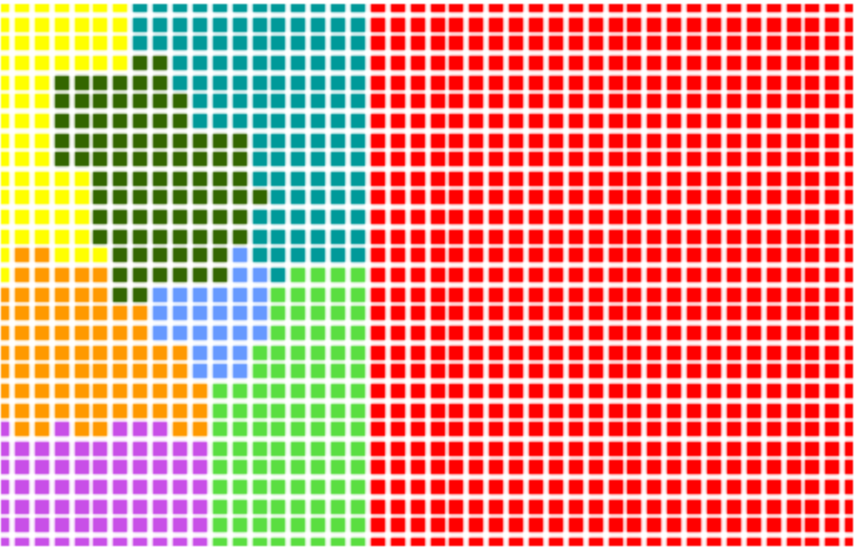
\includegraphics[width=0.7\textwidth]{images/discount4}}
    \caption[short]{partycjonowanie 3 z użyciem discountu}
\end{subfigure}
\caption{Obrazek (a) przedstawia siatkę wejściową, której więcej niż połowę zajmuje oznaczony kolorem żółtym obszar niepodzielny.
Obrazek (a), (b) oraz (c) przedstawia partycjonowanie siatki na 8 części wykonane algorytmem LAM bez fazy ulepszania podziału.
Obrazek (b) pokazuje partycjonowanie wykonane z użyciem warunku \ref{eq:condition1} na skojarzenie wierzchołków.
Obraz (c) oraz (d) prezentuję partycjonowanie wykonane z użyciem warunku \ref{eq:condition3}.}
\label{im:discount}
\end{figure}

\newpage
Negatywnym efektem stosowania $discountu$ jest większa liczba wywołań algorytmu LAM
- czasami zmienna $t$ musi urosnąć
do konkretnej wartości, umożliwiającej dokonanie kolejnych, blokowanych obecnie skojarzeń, a żadne inne skojarzenia,
które spełniałyby warunek nie są w danej chwili możliwe.
Rysunek \ref{im:discount} pokazuje pozytywne działanie modyfikacji na jakość podziału, wraz z porównaniem do poprzedniej
wersji warunku.

Skonstruowanie $discountu$ polegało na odpowiednim dobraniu jego wartości względem parametrów dzielonej siatki, tak by
nie działał zbyt agresywnie, nadmiernie przez to przedłużając obliczenia, ale jednocześnie był na tyle agresywny, aby pozwalał tylko na
kojarzenie wierzchołków prowadzące do możliwie równych podziałów.
Został skonstruowany na bazie podstawowego współczynnika $\frac{t}{T}$, który na podstawie wielu prób
dostosowałem dodatkowymi zmiennymi w poszukiwaniu wcześniej określonego balansu.
W momencie, w którym partycjonujemy obszar, w którym nie ma dużych obszarów niepodzielnych nie musimy stosować
$discountu$.
W takim wypadku jedynym jego efektem, będzie większa liczba wywołań algorytmu LAM.


